\documentclass{article}

% Language setting
% Replace `english' with e.g. `spanish' to change the document language
\usepackage[english]{babel}
\usepackage{indentfirst}
% Set page size and margins
% Replace `letterpaper' with `a4paper' for UK/EU standard size
\usepackage[letterpaper,top=2cm,bottom=2cm,left=3cm,right=3cm,marginparwidth=1.75cm]{geometry}

% Useful packages
\usepackage{amsmath}
\usepackage{graphicx}
\usepackage[colorlinks=true, allcolors=blue]{hyperref}
\usepackage{float}%稳定图片位置
\usepackage{graphicx,subfig}%画图

\title{Entrepreneurship in Blockchain for Medicine: \\A Case Study in Plastic Surgery}
\author{Chongdan Pan}

\begin{document}
\maketitle

\begin{abstract}
Plastic surgery is a hot market that growing quite quickly with tens of millions of surgical procedures performed every year all over the world. However, at present, it's not a well-regulated industry as well since there are many cases that patients are injured or die from malpractice. The malpractice may be caused by the uncertificated doctor or unqualified medicine. The intransparency of the market has greatly increased the risk of taking plastic surgery. In this paper, we proposed a case study with a system built upon blockchain. The system stores the patients' data as well as all actions that the patients and doctors take as traceable and immutable records. The sensitive and private information will be encrypted so that only the owners can manage them, while other parts of the record can be used to identify how previous surgeries are performed. Thanks to the smart contract, the system can also facilitate the process of medical claims and transactions.
\end{abstract}
\section{Introduction}
\subsection{Blockchain, Smart Contract and Decentralized Application}
\par Blockchain was introduced to the world as the fundamental technology of Bitcoin by Satoshi Nakamoto in 2008\cite{Bitcoin}. Designed to keep a record of every transaction in the system distributedly, blockchain has been proved to be reliable and robust in the past few years. It has resisted multiple network attacks and reached a total market value of 742 billion USD. The success of Bitcoin greatly inspired the world to apply blockchain to various areas, and keep exploiting more features from it.
\par The most important features of blockchain include but are not limited to anonymity, decentralization, transparency, and immutability. These features can not only be applied to a money system, but also any system where trust or privacy is required. Besides transaction history, blockchain is essentially capable of keeping the history and state of any system. The prosperity of NFT and Ethereum has proved that blockchain can lead to a consensus history of an artwork or the state of a Turning complete virtual machine.
\par, What's more, blockchain also leads to the applications of smart contract: "scripts that reside on the blockchain that allows for the automation of multi-step processes"\cite{SmartContract}. The smart contract provides a clear, flexible way for users to determine the future behavior of the system. The assurance and automation of a smart contract further eliminate the distrust between people and reduce the human effort in the system.
\par Decentralized application can be a higher layer built upon blockchain and smart contracts and they're developed in a certain blockchain programming language such as Solidity. Different from traditional applications, decentralized applications can run on a blockchain without a central authority, making it more robust. On the other hand, it provides a user-friendly interface for the user to access the function and data conveniently with features of blockchain being kept. Decentralized applications bridge the distance between users and blockchain, and boost entrepreneurship in the blockchain.
\subsection{Medicine and Cosmetic Surgery}
Medicine is an area where multiple parties are involved. Patients, doctors, hospitals, and manufacturers are key stakeholders who interact with each other in a complex way. In these intricate flows, trust is extremely critical because misbehaving or false information may put people's lives at risk. On the other hand, medicine and healthcare data are very sensitive because they're the private information of the patients. Entrepreneurship in blockchain for medicine can be very effective at solving these problems by reducing the requirement for trust and reinforcing the security of information.
\par Blockchain can have multiple applications in medicine, such as giving patients full control over their personal data or recording the information of drugs from supply chain \cite{Review}. It can also keep the important behavior of stakeholders so that people can know their reliability.
\par This paper specifically targets plastic surgery, a hot domain of medicine that is under rapid development. In 2020, over 24 million surgical procedures performed by more than 43750 surgeons were recorded by the International Society of Aesthetic Plastic Surgeries (ISAPS)\cite{ISAPS}. However, the industry is unregulated and in chaos, especially in some new markets like China. In 2019, the size of the medical aesthetics market in China amounted to 177 billion yuan, implying a yearly growth of 22 percent \cite{ChinaMarket}. However, there were only less than 24\% licensed doctors, and less than 12\% regulated institutions\cite{ChinaReport}. Underground plastic surgeries happen 
all over the world, and malpractice can lead to different outcomes including infection, disfigurement, or even death.
\par, In essence, it's the intransparency and information asymmetry that cause the chaos. Patients are so passionate about plastic surgeries but it's hard for them to know if the surgeon is certificated or if the medicine is approved for use. In this paper, we'll first analyze some solutions based on blockchain that can be applied to the plastic surgery industry. Then, we'll propose clean beauty, a digital system based on blockchain, support the transparent information flow and give patients full control of their own medical records. In the last part, we'll discuss the challenges of blockchain and its application for plastic surgery.

\section{Existing Solutions}
\subsection{Gem Health}
Gem Health is a decentralized application built upon a blockchain operating system GemOS\cite{Gem}. The start-up aims at using blockchain to create comprehensive medical histories for patients and improve the sharing of their data\cite{GemHealth}. By managing patients' data on the blockchain, the system can provide more accuracy, transparency, and accountability while maintaining patient privacy and HIPAA compliance\cite{GemBlog}. 
\begin{figure}[H]
    \centering
    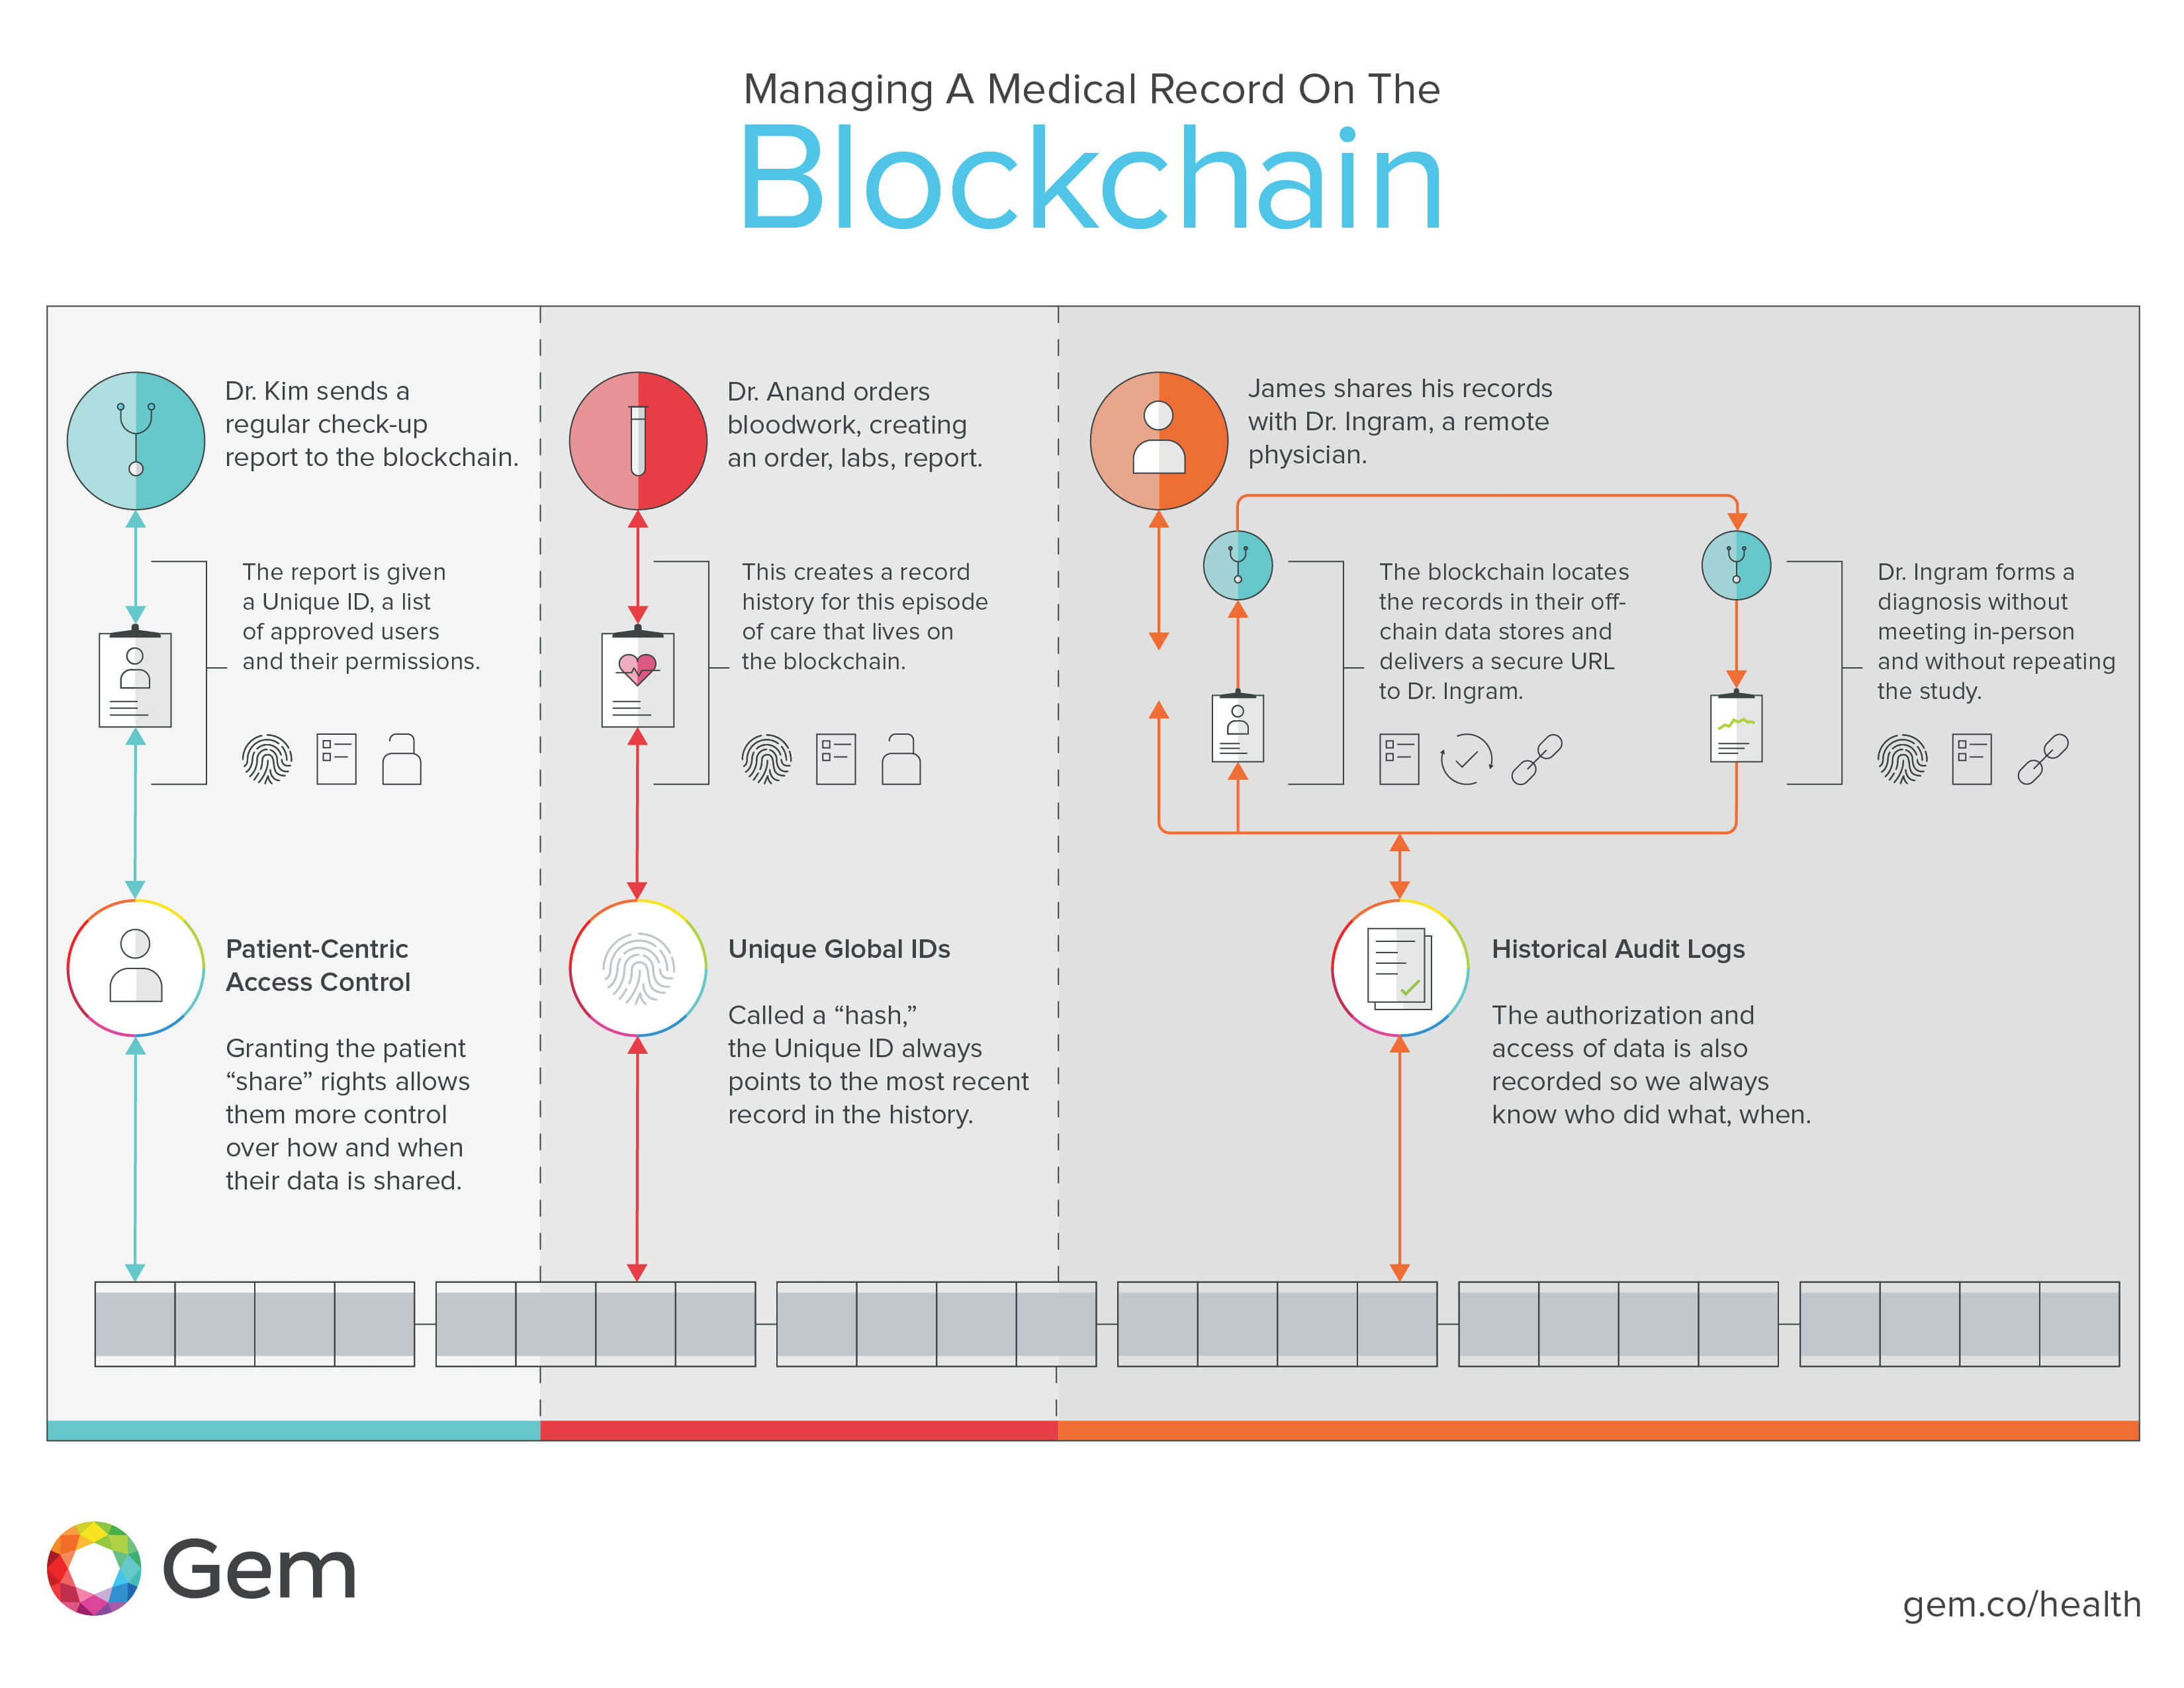
\includegraphics[scale=0.15]{GemBlockchain.jpg}
    \caption{Work flow of Gem Health System}
\end{figure}
The Gem Health system serves as a blockchain database of patients' data with permission control. When the doctor updated the health data to the blockchain, all information is recorded. The immutability and traceability of blockchain make it easier for people to check whether the data is valid and correct. On the other hand, with the public key and private key, the doctor and the patient can easily share their ownership in a peer-to-peer manner, so that only people with access and permission can view or modify the data. Since blockchain can be public, people granted access, can easily view the data without further communication. Blockchain makes the flow of patients' data much smoother and can save a lot of effort and time.
\par In addition to keeping patients' records, the system can also be applied to health claims\cite{GemClaims}. The Gem Health claims solution takes aims at facilitating three important processes. The real-time transparency during the claims, the amount of time it takes for providers to get paid for their service, and the rate of provider reimbursements. By keeping all-action regards to the transaction on the blockchain, people can transparently know how the claims procedure is executed, what the current stage is, and who is responsible for it right now. The efficiency of the reimbursements will also be improved because people don't have to take a long time to deliver or verify the claims information
\par, However, there are various challenges to the blockchain health system. How to get users aboard is very tricky, since people already have a huge amount of medical records which are hard to transfer. In some countries, the is a huge amount of privacy laws and healthcare workflow need to be adjusted to conform to the blockchain system. Not to mention that such a system will affect many people with vested interests such as electronic health record vendors and intermediaries.
\par, On the other hand, the performance of blockchain can also affect the scalability of the system. Ethereum, the most popular public blockchain for decentralized application, is suffering from the problem of congestion and high gas fee. Based on the blockchain trilemma, the scalability is limited when the system is pursuing high decentralization and security \cite{trilemma}. With more transactions running on the system, the limitation of scalability will not only raise the cost for the users but also increase the latency and affect the performance of features such as real-time transparency and reimbursements.
\subsection{Zocdoc}
Zocdoc is a streamlined system that provides patients with higher accessibility to doctors \cite{zocdoc}. When patients want to make a schedule with a doctor, the system can automatically provide a recommendation based on the patients' locations and other requirements. What's more, patients can publish their reviews for doctors on the application, which can be a good reference for other users. Then, patients and doctors can make an appointment for a further meeting. In plastic surgeries, the reviews can be extremely important for patients, because typically it's hard to know whether the doctor is certificated and how the surgery is conducted.
\par A common issue for Zocdoc is the reliability of the reviews. The doctor may post some fake reviews to raise the profile and attracts more customers. The phenomenon is very common in e-commerce platforms, where people can't trust the reviews anymore. Another major problem for Zocdoc is the patient may cancel or miss the appointment. As a result, the time of the clinic is lost and the revenue is decreased. Currently, Zocdoc will lock the patient's account if for multiple reschedules or cancellations, but the patient can avoid the side effect by setting up a new account. 
\section{Our solution for Plastic Surgery Industry}
\subsection{Introduction}
To solve the problems in the plastic surgery industry and medicine accessibility, we designed a system built upon blockchain, to make the process more transparent, reliable, and smooth for patients to get service from plastic surgeons. The blockchain can not only be used to manage the patient's health data or claims but also their interactions with doctors. In this way, all actions and reviews are recorded on the blockchain so that doctors and patients can know how reliable each other is by viewing the historical record. What's more, the blockchain can record the important information of prescription medicine to make sure they're qualified and safe.
\par Our system starts with the user proposing a smart contract to the doctor's public address. The confidential information of a smart contract will be encrypted, but the status of each smart and the public key of users will be public. Depending on what status a smart contract is, people's behavior can be traced. If a patient misses an appointment, then the smart contract cannot proceed to the next stage. Since the users' public key and status of each smart is public, the system can track how punctual the patient is. What's more, the smart contract ensures a seamless connection between data upload and payment. For example, the patient's medical history record will only be valid and stored on the blockchain when the user makes the necessary payment.
\subsection{Actors}
\subsubsection{Doctors}
Doctors are using the system to promote themselves and attract customers so that they can get great revenue from it. To get certificated and attractable for patients, the doctor needs to make important information public on the system, including digital identity and license. Since the license number is traceable, we can check whether the doctor is using a verified license or a fake one. The digital identity is like the public address or public key of the doctor. Patients can propose a smart contract and send the request to a doctor's public address. In addition, the patient can use the doctor's public key to encrypt the sensitive medical records and send them to the doctor. The transmission of the medical records will be recorded publicly on the blockchain, but its sensitive content is secure and only visible to the doctor thanks to the property of asymmetric encryption \cite{encryption}. The digital identity will be recorded on the blockchain with all actions that the doctor made, such as surgeries, prescriptions, examinations, and the review that the doctor got. Although the sensitive information in these actions is encrypted, people can still evaluate a doctor based on historical records and reviews.
\subsubsection{Patients}
Patients are other primary users of the system. The blockchain enables them to manage their data safely, as well as find reliable doctors based on the historical information stored on the blockchain. Before entering the system, the user needs to generate a public-private key pair. After the doctors' office visit, the doctor will use the public key to encrypt the patient's new medical history records and store them on the blockchain. In this way, only the patients and the doctor who uploaded the records can see the sensitive content. For doctors, they won't have any incentive to leak the information because people can easily check who may view the information and such action can injure the reputation. Hence, the patients have full control of the medical history records since nobody can see them later without the patient's private key. The patient's public key can be used to identify the patient as well since it represents the owners of the medical history records. Therefore, doctors can check the miss and reschedule rate of a patient as well be searching for the patient's historical actions on the blockchain.
\subsubsection{Third Parties}
Third parties can be other stakeholders or people who have an interest in the system, such as medicine manufacturers and insurance companies. A lot of plastic surgery malpractice is due to unqualified medicine, hence manufacturers will be asked to upload the serial number of medicine used in each prescription to the blockchain so that they can be verified and traceable. Storing the medicine information on the blockchain can also help the medicine manufacturers to manage the supply chain efficiently. For insurance companies, they can inject the insurance terms into the smart contract set between patients and doctors. With the help of a smart contract, the insurance can be more clearly identified and executed as automatically as possible.
\subsection{Workflow}
\begin{figure}[H]
    \centering
    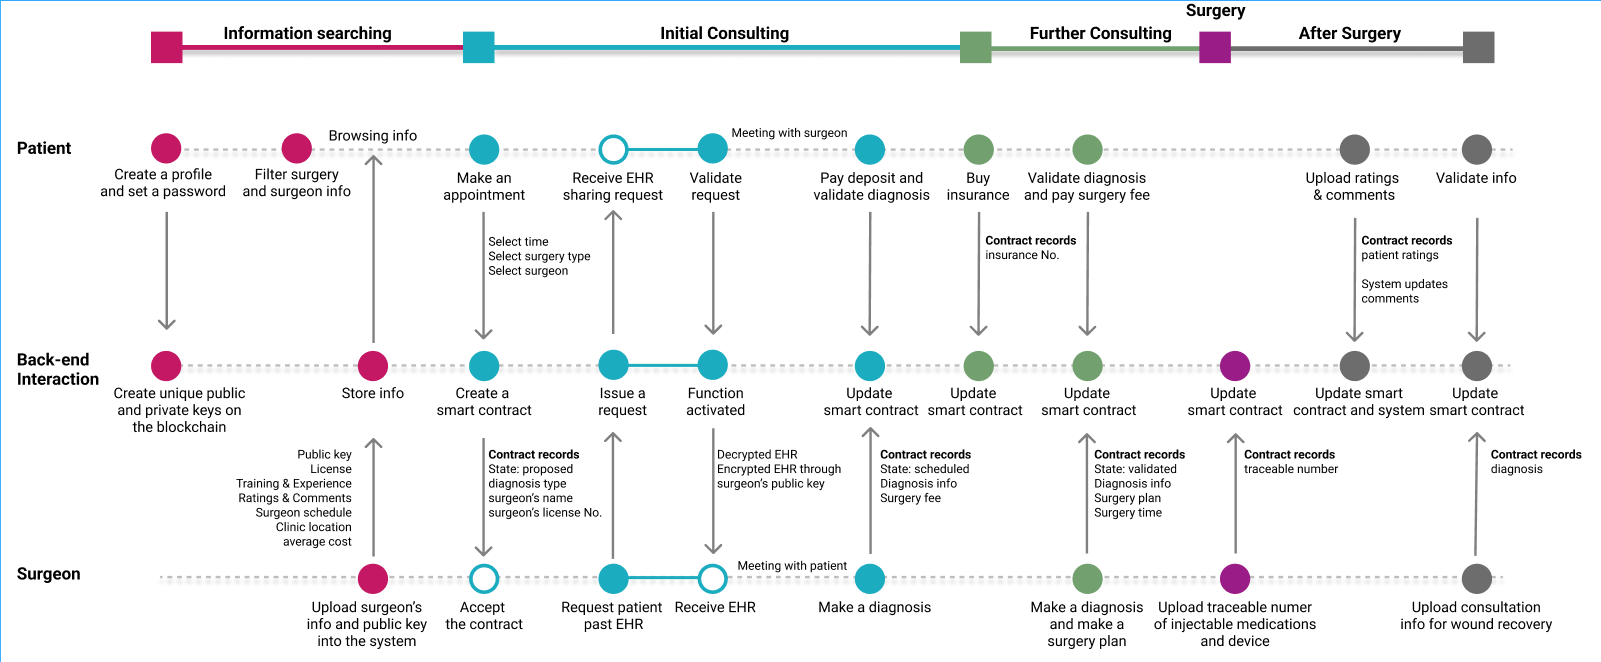
\includegraphics[scale=0.45]{Workflow.jpg}
    \caption{Example of our solution's work flow}
\end{figure}
The workflow between patients and doctors based on our system can be divided into four stages.
\subsubsection{Information Searching}
In this initial stage, patients and doctors need to create their private-public key pair so that the patient can set up a secure account to store health data and the doctor can become searchable. Then, the patient can search for doctors based on the initial public information stored on the blockchain.
\begin{figure}[H]
    \centering
    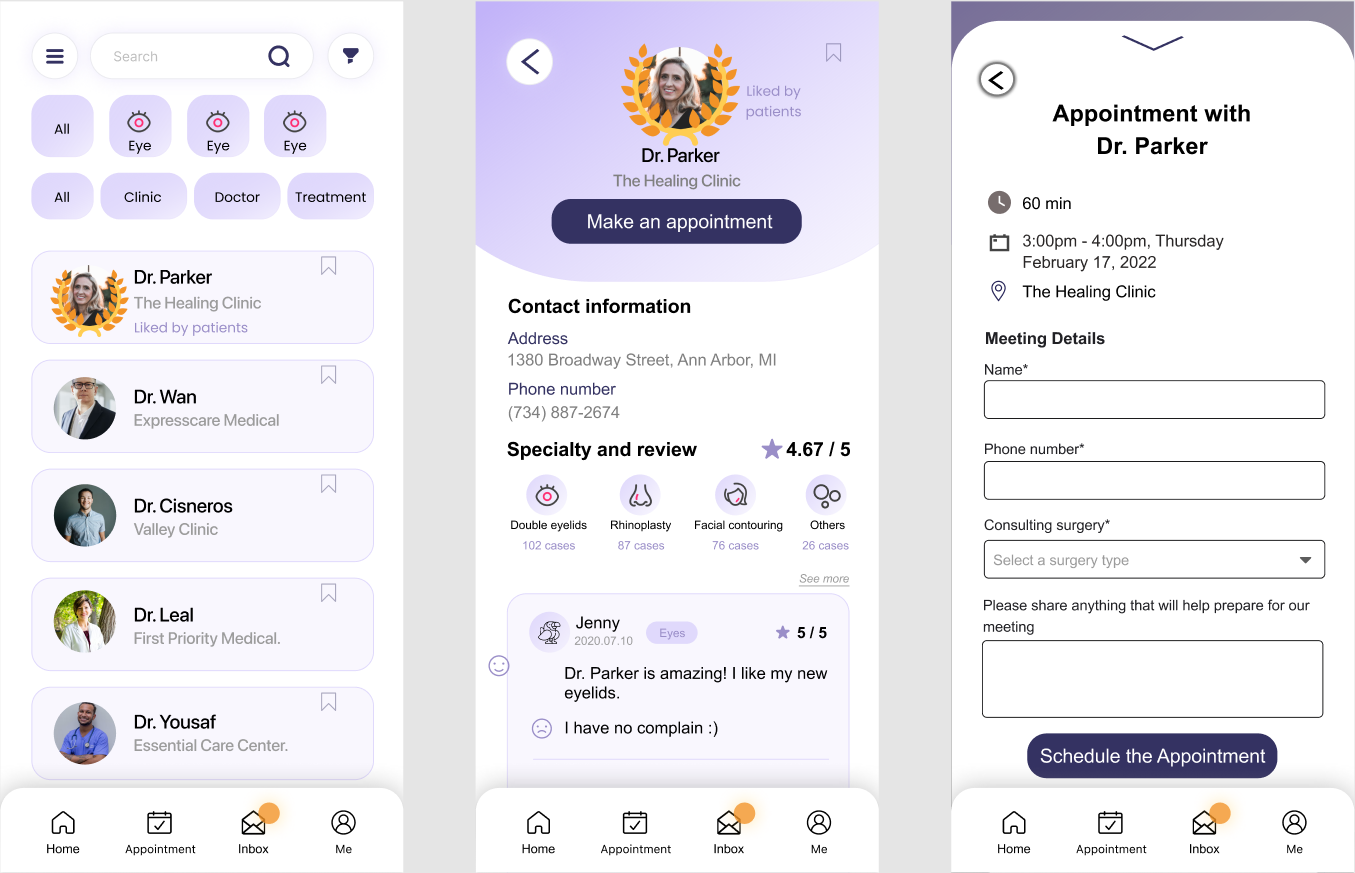
\includegraphics[scale=0.5]{Appointment.jpg}
    \caption{Information Search}
\end{figure}
The searching process is very similar to the existing application, and then the patient can propose a smart contract with an appointment time to the doctor's public address. The creation of a smart contract will cause some transaction fees since it needs to store new data on the blockchain. During the searching process, previous patients' reviews can serve as a reference. Users can make choices either based on the previous review or the smart contract records associated with a specific doctor. Different from the traditional system, it's impossible for the doctor to fake the review because they're linked to a  smart contract containing all immutable information regarding the treatment. If the doctor wants to make a fake review, he or she must go through the whole process from proposing a smart contract to the end of visiting, which requires a lot of time and money.
\subsubsection{Initial Consulting}
If the doctor accepted the smart contract by putting a digital signature on it, all basic information of patients and patients will be stored with it. Then the doctor can send a request for the patient's previous medical history record. Once received the request, only the patient who has the private key can determine whether to share it, because the medical history record is stored on the blockchain encrypted by the patient's key. If the patient authorizes the access, the records will be decrypted by the patient's key and encrypted by the doctors' key again so that only the doctor can view it.
\begin{figure}[H]
    \centering
    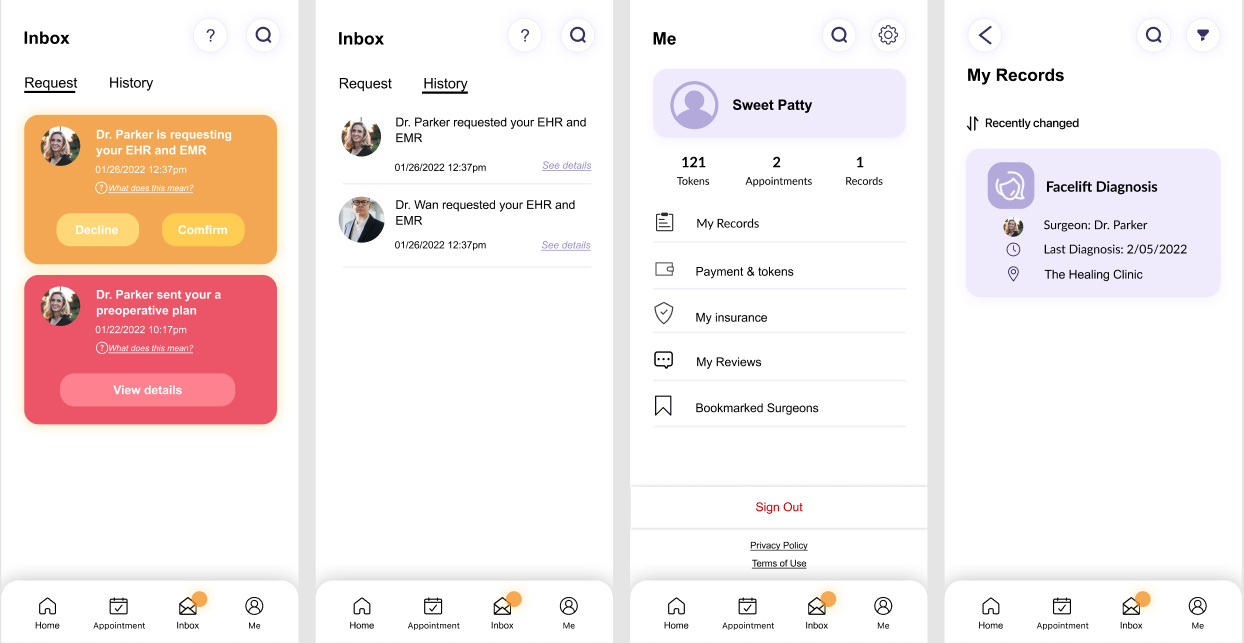
\includegraphics[scale=0.5]{InitialConsulting.jpg}
    \caption{Initial Consulting}
\end{figure}
\subsubsection{Further Consulting}
After the first consultation, doctors and patients should have a plan for the following surgery. In this stage, the smart contact can be linked to the insurance claims with clear terms. In this stage, the patient also needs to confirm the surgery plan by paying the deposit for it.
\begin{figure}[H]
    \centering
    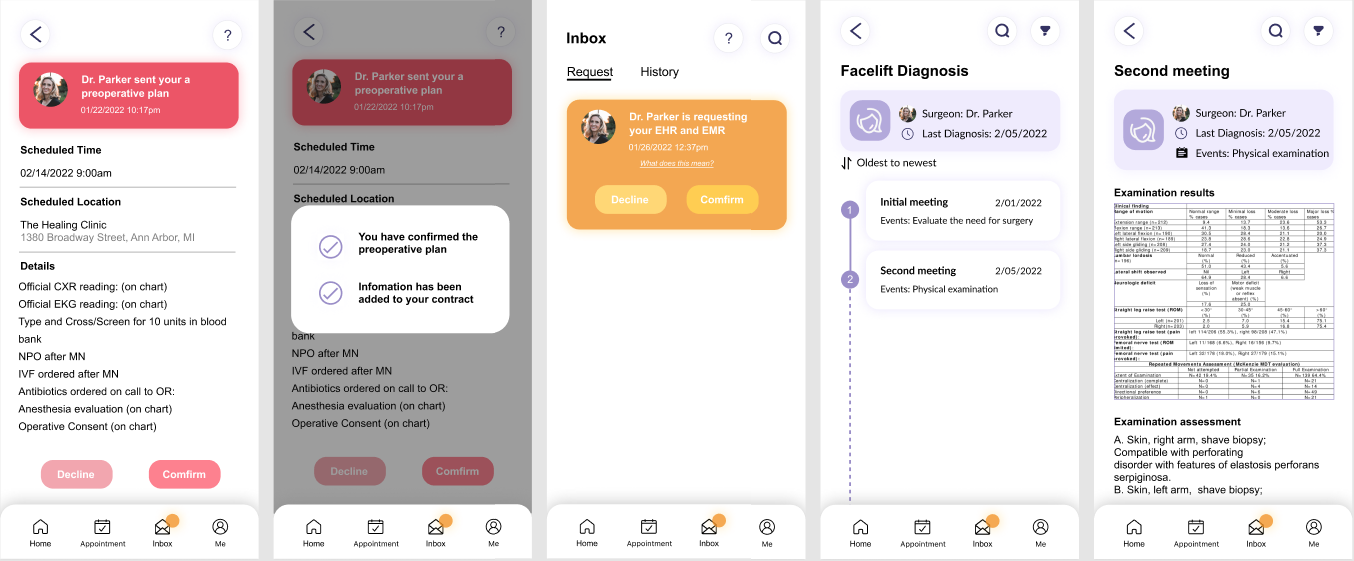
\includegraphics[scale=0.5]{SecondConsulting.jpg}
    \caption{Information Search}
\end{figure}
The surgery can proceed only after all previous diagnoses are verified and both the doctors and patients agree on the plan. All other medicine used in the surgery, such as anesthetics, should be recorded on the blockchain as well. Since everything is confirmed and recorded clearly, it'll be easy to track if there is something that happens with the surgery. 
\subsubsection{After surgery}
After the surgery, the doctor will encrypt the surgery summary and further prescription with the user's public key and upload the data on the blockchain. The smart contract will make sure that the data will only be valid after the user's confirmation and complete the transaction. The surgery summary will be designed to be structured so it can match well with the insurance term. If it matches any term, the smart contract will automatically execute it and proceed with the health claims.
\par When the patient's medical health records are validated, they will be encrypted and linked to the patient's public key, so that the patient can manage it later. In addition, the patient will be incentivized to provide a review for the doctor to help other patients make a choice.
\subsection{Challenges}
A major challenge for this system is how to be docked to the current medical system. Lots of people have their medical history records stored in the traditional system right now, and it'll take huge efforts to encrypt and upload them on the blockchain. The complexity of blockchain may also hinder users from using our system.
\par In the technology aspect, the system is designed to be running on a blockchain using Algorand consensus, which is claimed to be able to solve the blockchain trilemma with high scalability\cite{algorand}. However, due to the rapid development of blockchain technology, we think it will be helpful to set up a middle layer between our application with the layer-one solution like a virtual machine. In this way, the application and data can be easily transferred to a more advanced blockchain.
\par The volatility of blockchain tokens can be a challenge. Patients hope the cost for a surgery won't fluctuate all over time so that they can make a budget plan while the doctors want to get stable revenue. Since users of blockchain can't directly make payments through fiat currency, they need some way to make an exchange. One way to reduce volatility is to use stable tokens, but it also poses a challenge to control the issue of the token.
\par The complexity of smart contracts will make it challenging to set a standard way for it to proceed. Patients and doctors may have a disagreement on the status of a smart contract or what information should be considered as sensitive and need to be encrypted. The smart contract may lead to other problems that are hard to be solved by the law.
\section{Conclusion}
In this paper, we have an overview of the current plastic surgery industry and identify some problems and some existing solutions. Then we present a system built upon blockchain to make the industry more transparent, trustworthy, and efficient than ever. The immutability and traceability of the blockchain system make sure that everyone's action is recorded publicly so that patients can find reliable doctors and medicine based on previous records. Thanks to cryptography, the system also ensures the security of patient's private data. The smart contract makes the transaction between patients and doctors smoother and enables the automatic execution of insurance claims. The system is designed to reduce the requirement of trust between users and make the process automatically as much as possible. It's fully viable since it can be built upon existing technology. 
\bibliographystyle{plain}
\bibliography{Reference}

\end{document}